\documentclass[a4paper]{article}

\title{Ray Tracing}
\author{ab-gh}
\date{1 December 2021}

% LaTeX preambule: loading relevant packages, configuring Python listings
\usepackage{graphicx}
\usepackage{amsmath}
\usepackage{color}
\usepackage{listings}
\usepackage{hyperref}
\usepackage{bm}
\usepackage{amsfonts}
\usepackage{circuitikz}
\newcommand{\secref}[1]{\autoref{#1}. \nameref{#1}}

\usepackage[a4paper, total={6in, 8in}]{geometry}

\definecolor{dkgreen}{rgb}{0,0.6,0}
\definecolor{gray}{rgb}{0.5,0.5,0.5}
\definecolor{mauve}{rgb}{0.58,0,0.82}

% Settings for colour-coding and formatting Python code:
\lstset{
  language=Python,                % the language of the code
  basicstyle=\ttfamily\footnotesize,           % the size of the fonts that are used for the code
  numbers=left,                   % where to put the line-numbers
  numberstyle=\tiny\color{gray},  % the style that is used for the line-numbers
  stepnumber=5,                   % the step between two line-numbers. If it's 1, each line
                                  % will be numbered
  numbersep=5pt,                  % how far the line-numbers are from the code
  backgroundcolor=\color{white},      % choose the background color. You must add \usepackage{color}
  showspaces=false,               % show spaces adding particular underscores
  showstringspaces=false,         % underline spaces within strings
  showtabs=false,                 % show tabs within strings adding particular underscores
  frame=single,                   % adds a frame around the code
  rulecolor=\color{black},        % if not set, the frame-color may be changed on line-breaks within not-black text (e.g. commens (green here))
  tabsize=2,                      % sets default tabsize to 2 spaces
  captionpos=b,                   % sets the caption-position to bottom
  breaklines=true,                % sets automatic line breaking
  breakatwhitespace=false,        % sets if automatic breaks should only happen at whitespace
  title=\lstname,                   % show the filename of files included with \lstinputlisting;
                                  % also try caption instead of title
  keywordstyle=\color{blue},          % keyword style
  commentstyle=\color{dkgreen},       % comment style
  stringstyle=\color{mauve},         % string literal style
  escapeinside={\%*}{*)},            % if you want to add LaTeX within your code
  morekeywords={*,...}               % if you want to add more keywords to the set
}

\begin{document}
\maketitle

{\bf Task:} To create an advanced optical simulation program in C++. Using the principles of {\it Ray Tracing}, {\it Object-Oriented Design}, and the material covered in PH3170, this project aims to produce a realistic image of a simulated scene, including accurate objects and lighting.

\section{Introduction and Theory}
To start the project, I set out a series of objectives for the final code, and a set of milestones to progress through. In order to fulfill the requirements of the task, my code needs to be able to:
\begin{itemize}
  \item{Allow a user to specify the geometry, location, and material properties of primative shapes in the scene.}
  \item{Allow a user to specify the location and intensity of sources of light.}
  \item{Simulate the object's interactions with the light sources and other objects in the scene using {\it reverse ray tracing}.}
  \item{Produce an image of the simulated scene, as if a camera was taking a photograph.}
\end{itemize}
To achieve these aims, I set out to complete the following milestones, roughly in order. By breaking the project down into smaller components, I not only ensure that I don't waste time working on one feature when an underlying feature is broken, but also lend my code-writing process to Object Oriented Design (OOD) principles.
\begin{enumerate}
  \item{Construct a fully-functional but abstract Vector data type, capable of defining vectors and points in 3D cartesian space, and computing all relevant vector operations.}
  \item{Construct a ``virtual camera'', which sends rays out into the ``world''.}
  \item{Define primative objects, classes which contain the object's geometry and properties, as well as functions to calculate the intersections between its self and a camera ray, and a function to calculate the surface normal of the shape at any point.}
  \item{Define light sources, with an intensity and position.}
  \item{Construct a ``rendering engine'', capable of simulating various types of illumination, and linking the virtual camera to the ``world'' (scene) of objects in front of it.}
\end{enumerate}
\subsection{Ray Tracing Theory}
To produce a realistic depiction of the scene, this project uses a technique called {\it reverse ray tracing}. In a real physical scene, the illumination of objects can be approximated as light sources emitting rays which interact with the object, reflecting light to a new ray direction. If one of these light rays, after however many reflections, hits a sensor (be it an eye or camera), it is ``seen'' by the observer. In a computational simulation, a tiny fraction of the rays emitted from a source will actually make it to the observer, so this process is very inefficient.

To combat this, {\it reverse} ray tracing is used, with the same principles, except the observer emits a ``sight'' ray, which reflects according to the same laws, until it hits a light source. To produce the image, the observer ``looks'' through a viewport - a rectangular boundary in space - similarly to a camera sensor. Sight rays are constructed with a vector from an ``eye'' (focus of the observation plane) to each pixel on the viewport, which is then projected into the scene, and the reverse ray tracing begins.

\begin{figure}[!h]
  \centering
  \begin{circuitikz}
    \draw [line width=0.5mm] (0,0) node {} -- (0,3) node[pos=1,above] {viewport};
    \draw (5,0) circle (1cm);
    \draw[fill=black] (-2,1.5) circle (0.1cm);
    \draw[fill=yellow] (3,2.9) circle (0.1cm);
    \draw (-2,1.5) node[above left=of eye] {eye} to node[currarrow] {} (4.2,0.6);
    \draw[->] (4.2,0.6) -- (3.5,1.125) node[above left=of $\hat n$] {$\hat n$};
    \draw (4.2,0.6) node to node[curarrow] {} (3,2.9) node[above right=of light source] {light source};
  \end{circuitikz}
  \caption{Demonstration of reverse ray tracing, reflecting a sight ray from the eye through the viewport off a sphere.}
\end{figure}

\subsection{Object Oriented Design}
This project required a lot of different components to work together accurately, yet still abstract enough to be flexible, allowing the development of more shapes, interactions, and materials in future. Because of this, applying the principles of Object Oriented Design was essential. Each component of the project was ``compartmentalized'' in its own header file, using inheritance where possible. Each class interacts with the renderer, which produces the final image.

\section{Implementation}
This section explains the implementation of the ray tracing simulator, following the process outline in the milestones above.

\subsection{Vector base class}
The first task of the implementation was to construct a fully-featured vector class. Defined in \verb|Vector.h|, the \verb|Vector| class serves as the basis for almost every other element of the simulator. As such, it defines an extensive list of methods and operations for vectors.
% dont need all of these vector sections %

\begin{lstlisting}[language=C++, belowskip=-0.8 \baselineskip]
class Vector {
  private:
      double vector[3];
  public:
      Vector() : vector{0, 0, 0} {};
      Vector(double x, double y, double z) : vector{x, y, z} {};
      ...
  };
\end{lstlisting}Operations for vectors are also defined outside of the \verb|Vector| class, as inline functions, so that they can be accessed outside of a Vector:
\begin{lstlisting}[language=C++, belowskip=-0.8 \baselineskip]
inline Vector operator+(const Vector &u, const Vector &v) {
    return {u.x() + v.x(), u.y() + v.y(), u.z() + v.z()};
}
...
\end{lstlisting}In addition to the basic mathematical operations, the header file defines the dot and cross product (\verb|dot(u,v)|, \verb|cross(u,v)|), unit vector (\verb|unit(u)|), as well as reflections (\verb|reflect(i,n)|) and refractions (\verb|refract(i,n,eta)|). The \verb|Vector| class also has three aliases, which help to make their specific use clearer in context: \verb|V3|, \verb|P3|, \verb|RGB|.

RGB vectors have their own class definition, \verb|RGB.h|. These force the values to be ``clamped'' between 0 and 255 when output, and provide a \verb|write_RGB| function to write an RGB value out to a file.

\subsection{Camera, viewport, and scene}
Now that the basic vector class is implemented, the virtual world of the simulation can be built. The file \verb|Camera.h| defines the \verb|Camera| class, which includes the eye and viewport. For simplicity, this has default values of a 16:9 aspect ratio image, with 1000 pixels across, which translates to a height of $2$ in the simulated world. The focal length is defined as $1$, which means the ``eye'' is one unit behind the centre of the viewport. The viewport is centered on the origin, looking down the negative $z$ axis. This geometry allows you to consider the image as if it were an $x,y$ plane, with depth as $-z$. 

Next, the \verb|Scene.h| file defines the simulated world as the class \verb|Scene|. This is a very simple class, with two \verb|std::vector| attributes: one to hold the list of objects in the scene, and one to hold the list of light sources. Two methods - \verb|addObject()| and \verb|addSource()| are also defined, which add objects and light sources to the scene once created.

\verb|Scene.h| also defines \verb|save()| and \verb|read()| methods, which save the existing scene to a ``scene'' file, or load in a generated scene file. These allow for complex scenes to be defined without creating a complex \verb|main.cpp| file, or allow a ``base'' world (such as a basic room with soft lighting) to be imported, and extra objects added (as in the demonstration \verb|main.cpp|).

\verb|Ray.h| defines the aforementioned ``sight''-rays. It is a very simple class, defining a ray as having a vector origin and unit vector direction. It also defines a \verb|()| operator, which allows the calculation of a ray at ``time'' $t$ or ``distance'' $\mu$ much like one would define a function: \verb|Ray(x)|.

\subsection{Objects, intersections, and normals}
With a class now defined to hold objects in a world, the next step was to define those objects. To render an object in the world, each object class requires a series of defining parameters (which can define a unique instance of the object), and two methods: one to calculate where a vector line will intersect with the object's surface, and one to calculate the normal to the object's surface at any point. If these two functions are provided, the surface of any object can be detected and rendered by the renderer.

\verb|Object.h| defines several different objects to choose from, as well as an abstract base class used to build the other objects. \verb|Object| class defines the functions needed for an object: a parameter constructor, a string constructor (used to deserialize information when calling \verb|Scene.read()|), an intersection function, a normal function, and a serializer (for \verb|Scene.save()|). One feature of note is the return type of the \verb|Object.intersect()| function. This function returns a pair \verb|std::pair<double, const Object*>|, where the double is the unit direction multiplier of the ray's intersection point. While it may seem redundant to return the object that has been intersected, this allows complex objects to be created with ``sub-objects''. For instance, the \verb|Cone| object is comprised of an ``empty'' cone, with a base cap, which is actually a \verb|Disc| sub-object.

This project currently implements the following shapes:
\begin{itemize}
  \item \verb|Sphere|
  \begin{itemize}
    \item \verb|Vector| position
    \item \verb|double| radius
    \item \verb|Vector| colour
    \item \verb|double| reflectivity
  \end{itemize}
  \item \verb|InfinitePlane|
  \begin{itemize}
    \item \verb|Vector| position
    \item \verb|Vector| normal
    \item \verb|Vector| colour
    \item \verb|double| reflectivity
  \end{itemize}
  \item \verb|Disc|
  \begin{itemize}
    \item \verb|Vector| position
    \item \verb|Vector| normal
    \item \verb|double| radius
    \item \verb|Vector| colour
    \item \verb|double| reflectivity
  \end{itemize}
  \item \verb|Cone|
  \begin{itemize}
    \item \verb|Vector| position
    \item \verb|Vector| base
    \item \verb|double| radius
    \item \verb|Vector| colour
    \item \verb|double| reflectivity
  \end{itemize}
\end{itemize}

\subsection{Sources and intensity}
Now that objects can be defined, light sources need to be provided to allow them to be illuminated. These are defined in \verb|Source.h|, which defines a \verb|Source| class. This requires a position and intensity, and provides a deserialization constructor and a serializer. While only invisible point-sources are defined, it would be easy to extend this class to create visible sources (i.e. emissive objects) with intersection and normal functions, or different light sources such as a ``sun'' (i.e. a source at infinity with parallel light rays) or a directional light (i.e. a source which only provides illumination at some solid angle). 

\subsection{Rendering and Image Generation}
The final - and by far the most complex - requirement for the project is the ``rendering engine''. This is defined in \verb|Render.h| and, while not a class, defines a multitude of functions. Below is a simple flowchart describing the operation of the rendering engine.

\begin{figure}[!h]
\centering
\tikzset{every picture/.style={line width=0.75pt}} %set default line width to 0.75pt        
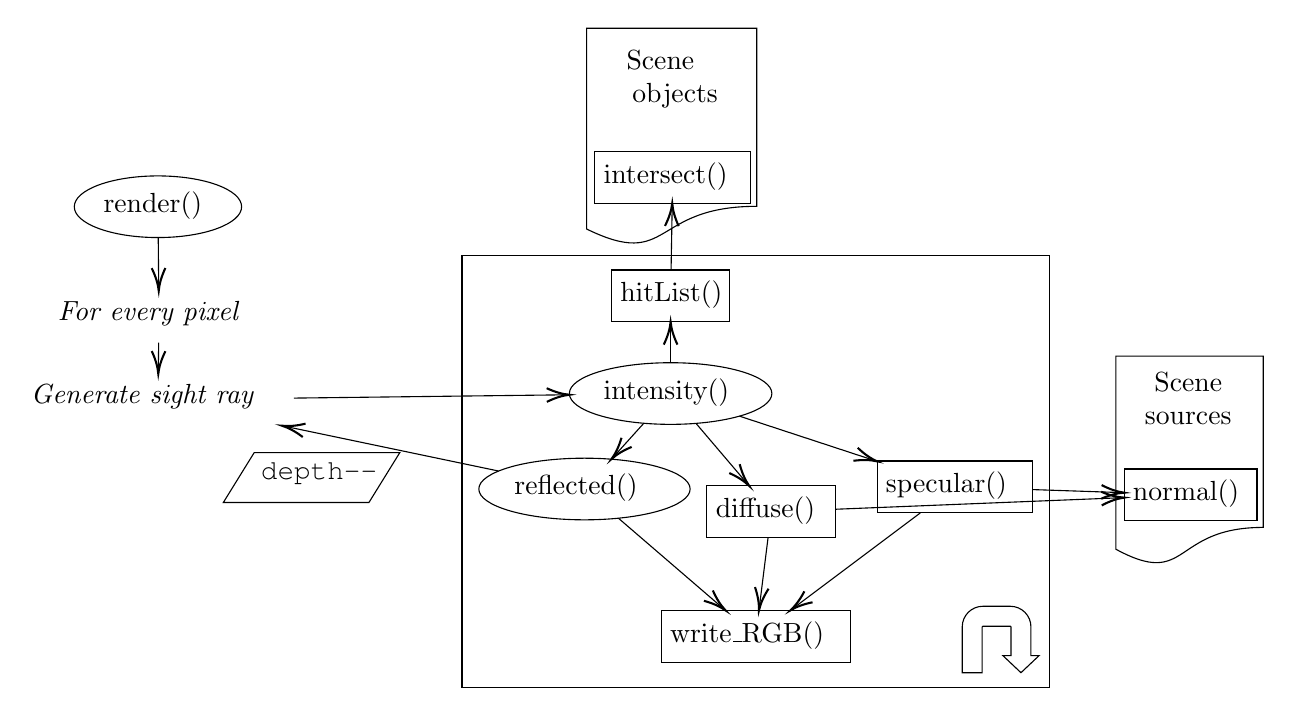
\begin{tikzpicture}[x=0.75pt,y=0.75pt,yscale=-1,xscale=1]
%uncomment if require: \path (0,533); %set diagram left start at 0, and has height of 533

%Shape: Rectangle [id:dp36562694200461954] 
\draw   (271,244) -- (554,244) -- (554,452) -- (271,452) -- cycle ;
%Shape: Parallelogram [id:dp4553637708711975] 
\draw   (170.85,339) -- (241,339) -- (226.15,363) -- (156,363) -- cycle ;
%U Turn Arrow [id:dp7755308375832675] 
\draw   (512,445) -- (512,422.93) .. controls (512,417.45) and (516.45,413) .. (521.93,413) -- (535.17,413) .. controls (540.66,413) and (545.1,417.45) .. (545.1,422.93) -- (545.1,436.79) -- (549,436.79) -- (540.3,445) -- (531.61,436.79) -- (535.5,436.79) -- (535.5,422.93) .. controls (535.5,422.75) and (535.36,422.6) .. (535.17,422.6) -- (521.93,422.6) .. controls (521.75,422.6) and (521.6,422.75) .. (521.6,422.93) -- (521.6,445) -- cycle ;
%Flowchart: Document [id:dp13007814499197756] 
\draw   (331,134.5) -- (413,134.5) -- (413,220.3) .. controls (361.75,220.3) and (372,251.24) .. (331,231.22) -- cycle ;
%Flowchart: Document [id:dp7707050305878355] 
\draw   (586,292.5) -- (657,292.5) -- (657,375) .. controls (612.63,375) and (621.5,404.75) .. (586,385.5) -- cycle ;

% Text Node
\draw    (124.5, 220.5) circle [x radius= 40.31, y radius= 14.85]   ;
\draw (97,212) node [anchor=north west][inner sep=0.75pt]   [align=left] {render()};
% Text Node
\draw    (371.5, 310.5) circle [x radius= 48.79, y radius= 14.85]   ;
\draw (338,302) node [anchor=north west][inner sep=0.75pt]   [align=left] {intensity()};
% Text Node
\draw    (343,251) -- (400,251) -- (400,276) -- (343,276) -- cycle  ;
\draw (346,255) node [anchor=north west][inner sep=0.75pt]   [align=left] {hitList()};
% Text Node
\draw  [fill={rgb, 255:red, 255; green, 255; blue, 255 }  ,fill opacity=1 ]  (471,343) -- (546,343) -- (546,368) -- (471,368) -- cycle  ;
\draw (474,347) node [anchor=north west][inner sep=0.75pt]   [align=left] {\textcolor[rgb]{0,0,0}{specular()}};
% Text Node
\draw    (389,355) -- (451,355) -- (451,380) -- (389,380) -- cycle  ;
\draw (392,359) node [anchor=north west][inner sep=0.75pt]   [align=left] {diffuse()};
% Text Node
\draw    (330, 356.5) circle [x radius= 50.91, y radius= 14.85]   ;
\draw (295,348) node [anchor=north west][inner sep=0.75pt]   [align=left] {reflected()};
% Text Node
\draw (75,265) node [anchor=north west][inner sep=0.75pt]   [align=left] {\textit{For every pixel}};
% Text Node
\draw (62,305) node [anchor=north west][inner sep=0.75pt]   [align=left] {\textit{Generate sight ray}};
% Text Node
\draw    (367,415) -- (458,415) -- (458,440) -- (367,440) -- cycle  ;
\draw (370,419) node [anchor=north west][inner sep=0.75pt]   [align=left] {write\_RGB()};
% Text Node
\draw (172.85,342) node [anchor=north west][inner sep=0.75pt]   [align=left] {{\fontfamily{pcr}\selectfont depth--}};
% Text Node
\draw (349,144) node [anchor=north west][inner sep=0.75pt]   [align=left] {\begin{minipage}[lt]{35.04pt}\setlength\topsep{0pt}
Scene
\begin{center}
objects
\end{center}

\end{minipage}};
% Text Node
\draw (594,299) node [anchor=north west][inner sep=0.75pt]   [align=left] {\begin{minipage}[lt]{38.44pt}\setlength\topsep{0pt}
\begin{center}
Scene\\sources
\end{center}

\end{minipage}};
% Text Node
\draw    (335,193.86) -- (410,193.86) -- (410,218.86) -- (335,218.86) -- cycle  ;
\draw (338,197.86) node [anchor=north west][inner sep=0.75pt]   [align=left] {intersect()};
% Text Node
\draw    (590,346.86) -- (654,346.86) -- (654,371.86) -- (590,371.86) -- cycle  ;
\draw (593,350.86) node [anchor=north west][inner sep=0.75pt]   [align=left] {normal()};
% Connection
\draw    (371.5,295.65) -- (371.5,278) ;
\draw [shift={(371.5,276)}, rotate = 90] [color={rgb, 255:red, 0; green, 0; blue, 0 }  ][line width=0.75]    (10.93,-3.29) .. controls (6.95,-1.4) and (3.31,-0.3) .. (0,0) .. controls (3.31,0.3) and (6.95,1.4) .. (10.93,3.29)   ;
% Connection
\draw    (404.66,321.39) -- (469.1,342.56) ;
\draw [shift={(471,343.18)}, rotate = 198.18] [color={rgb, 255:red, 0; green, 0; blue, 0 }  ][line width=0.75]    (10.93,-3.29) .. controls (6.95,-1.4) and (3.31,-0.3) .. (0,0) .. controls (3.31,0.3) and (6.95,1.4) .. (10.93,3.29)   ;
% Connection
\draw    (383.73,324.88) -- (408.07,353.48) ;
\draw [shift={(409.36,355)}, rotate = 229.61] [color={rgb, 255:red, 0; green, 0; blue, 0 }  ][line width=0.75]    (10.93,-3.29) .. controls (6.95,-1.4) and (3.31,-0.3) .. (0,0) .. controls (3.31,0.3) and (6.95,1.4) .. (10.93,3.29)   ;
% Connection
\draw    (358.58,324.82) -- (344.3,340.65) ;
\draw [shift={(342.96,342.14)}, rotate = 312.06] [color={rgb, 255:red, 0; green, 0; blue, 0 }  ][line width=0.75]    (10.93,-3.29) .. controls (6.95,-1.4) and (3.31,-0.3) .. (0,0) .. controls (3.31,0.3) and (6.95,1.4) .. (10.93,3.29)   ;
% Connection
\draw    (124.64,235.35) -- (124.86,259) ;
\draw [shift={(124.88,261)}, rotate = 269.46] [color={rgb, 255:red, 0; green, 0; blue, 0 }  ][line width=0.75]    (10.93,-3.29) .. controls (6.95,-1.4) and (3.31,-0.3) .. (0,0) .. controls (3.31,0.3) and (6.95,1.4) .. (10.93,3.29)   ;
% Connection
\draw    (124.84,286) -- (124.68,299) ;
\draw [shift={(124.66,301)}, rotate = 270.72] [color={rgb, 255:red, 0; green, 0; blue, 0 }  ][line width=0.75]    (10.93,-3.29) .. controls (6.95,-1.4) and (3.31,-0.3) .. (0,0) .. controls (3.31,0.3) and (6.95,1.4) .. (10.93,3.29)   ;
% Connection
\draw    (190,312.7) -- (320.75,311.12) ;
\draw [shift={(322.75,311.09)}, rotate = 179.3] [color={rgb, 255:red, 0; green, 0; blue, 0 }  ][line width=0.75]    (10.93,-3.29) .. controls (6.95,-1.4) and (3.31,-0.3) .. (0,0) .. controls (3.31,0.3) and (6.95,1.4) .. (10.93,3.29)   ;
% Connection
\draw    (288.63,347.84) -- (186.2,326.41) ;
\draw [shift={(184.24,326)}, rotate = 11.82] [color={rgb, 255:red, 0; green, 0; blue, 0 }  ][line width=0.75]    (10.93,-3.29) .. controls (6.95,-1.4) and (3.31,-0.3) .. (0,0) .. controls (3.31,0.3) and (6.95,1.4) .. (10.93,3.29)   ;
% Connection
\draw    (346.35,370.57) -- (396.46,413.7) ;
\draw [shift={(397.98,415)}, rotate = 220.72] [color={rgb, 255:red, 0; green, 0; blue, 0 }  ][line width=0.75]    (10.93,-3.29) .. controls (6.95,-1.4) and (3.31,-0.3) .. (0,0) .. controls (3.31,0.3) and (6.95,1.4) .. (10.93,3.29)   ;
% Connection
\draw    (418.44,380) -- (414.31,413.02) ;
\draw [shift={(414.06,415)}, rotate = 277.13] [color={rgb, 255:red, 0; green, 0; blue, 0 }  ][line width=0.75]    (10.93,-3.29) .. controls (6.95,-1.4) and (3.31,-0.3) .. (0,0) .. controls (3.31,0.3) and (6.95,1.4) .. (10.93,3.29)   ;
% Connection
\draw    (491.83,368) -- (430.77,413.8) ;
\draw [shift={(429.17,415)}, rotate = 323.13] [color={rgb, 255:red, 0; green, 0; blue, 0 }  ][line width=0.75]    (10.93,-3.29) .. controls (6.95,-1.4) and (3.31,-0.3) .. (0,0) .. controls (3.31,0.3) and (6.95,1.4) .. (10.93,3.29)   ;
% Connection
\draw    (371.72,251) -- (372.25,220.86) ;
\draw [shift={(372.28,218.86)}, rotate = 91] [color={rgb, 255:red, 0; green, 0; blue, 0 }  ][line width=0.75]    (10.93,-3.29) .. controls (6.95,-1.4) and (3.31,-0.3) .. (0,0) .. controls (3.31,0.3) and (6.95,1.4) .. (10.93,3.29)   ;
% Connection
\draw    (546,356.78) -- (588,358.2) ;
\draw [shift={(590,358.27)}, rotate = 181.95] [color={rgb, 255:red, 0; green, 0; blue, 0 }  ][line width=0.75]    (10.93,-3.29) .. controls (6.95,-1.4) and (3.31,-0.3) .. (0,0) .. controls (3.31,0.3) and (6.95,1.4) .. (10.93,3.29)   ;
% Connection
\draw    (451,366.25) -- (588,360.73) ;
\draw [shift={(590,360.65)}, rotate = 177.69] [color={rgb, 255:red, 0; green, 0; blue, 0 }  ][line width=0.75]    (10.93,-3.29) .. controls (6.95,-1.4) and (3.31,-0.3) .. (0,0) .. controls (3.31,0.3) and (6.95,1.4) .. (10.93,3.29)   ;
\end{tikzpicture}

\caption{Flowchart describing the operation of the rendering engine.}
\end{figure}

When the \verb|render()| function is called, and is passed a valid scene and camera, it will loop over each pixel in the viewport and construct a ray from the ``eye'' to that pixel. It then projects the ray into the scene, and follows a process to determine the pixel's colour:
\begin{enumerate}
  \item For each object in the scene's object list, find where the ray intersects the object.
  \item For the closest object, calculate the intensity by summing, for each source:
  \begin{itemize}
    \item Diffuse illumination, by taking the dot product of the vector from the intersection point to the source, with the surface normal at the intersection point.
    \item Specular illumination, by taking the dot product of the vector from the intersection point to the source, with the reflected ray around the surface normal at the intersection point.
    \item Reflective illumination, by taking the reflected ray around the surface normal at the intersection point, and treating that as a new sight ray, projecting it into the scene, and going to step 2.
  \end{itemize}
  \item Write the pixel's RGB values out to the i
  mage file.
\end{enumerate}
To generate each ``sight'' ray, the renderer creates vectors from the lower-left corner of the viewport along the $x$ and $y$ axis to the pixel. As the renderer also knows the vector from the origin to the eye, and the origin to the lower-left corner, it can construct a vector from the eye to the pixel. That vector is then used to define the sight ray's direction, and the eye is used as the origin. This is shown below in Figure 3.

\begin{figure}[!h]
  \centering



  \tikzset{every picture/.style={line width=0.75pt}} %set default line width to 0.75pt        

  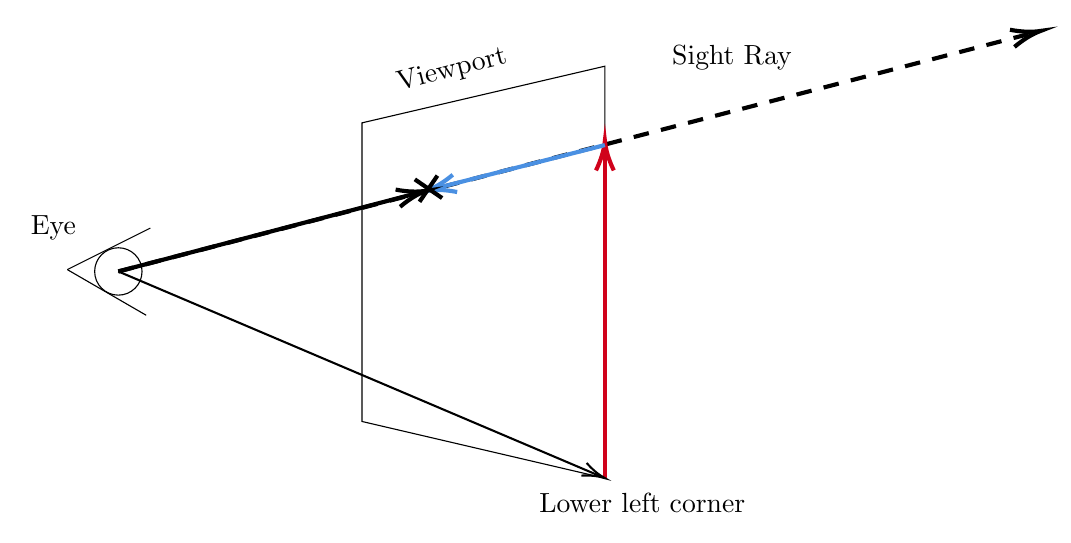
\begin{tikzpicture}[x=0.75pt,y=0.75pt,yscale=-1,xscale=1]
  %uncomment if require: \path (0,300); %set diagram left start at 0, and has height of 300
  
  %Straight Lines [id:da17863768780114508] 
  \draw [color={rgb, 255:red, 0; green, 0; blue, 0 }  ,draw opacity=1 ][line width=1.5]  [dash pattern={on 5.63pt off 4.5pt}]  (165.41,140.41) -- (606.93,25.28) ;
  \draw [shift={(609.83,24.52)}, rotate = 165.38] [color={rgb, 255:red, 0; green, 0; blue, 0 }  ,draw opacity=1 ][line width=1.5]    (14.21,-4.28) .. controls (9.04,-1.82) and (4.3,-0.39) .. (0,0) .. controls (4.3,0.39) and (9.04,1.82) .. (14.21,4.28)   ;
  %Shape: Trapezoid [id:dp1174799712357697] 
  \draw   (399.83,240) -- (282.83,212.7) -- (282.83,68.82) -- (399.83,41.52) -- cycle ;
  %Shape: Circle [id:dp4165673384186185] 
  \draw   (154,140.41) .. controls (154,134.11) and (159.11,129) .. (165.41,129) .. controls (171.72,129) and (176.83,134.11) .. (176.83,140.41) .. controls (176.83,146.72) and (171.72,151.83) .. (165.41,151.83) .. controls (159.11,151.83) and (154,146.72) .. (154,140.41) -- cycle ;
  %Straight Lines [id:da432002112670936] 
  \draw [color={rgb, 255:red, 208; green, 2; blue, 27 }  ,draw opacity=1 ][line width=1.5]    (399.83,240) -- (399.83,80.52) ;
  \draw [shift={(399.83,77.52)}, rotate = 90] [color={rgb, 255:red, 208; green, 2; blue, 27 }  ,draw opacity=1 ][line width=1.5]    (14.21,-4.28) .. controls (9.04,-1.82) and (4.3,-0.39) .. (0,0) .. controls (4.3,0.39) and (9.04,1.82) .. (14.21,4.28)   ;
  %Straight Lines [id:da05467739122704984] 
  \draw [color={rgb, 255:red, 74; green, 144; blue, 226 }  ,draw opacity=1 ][line width=1.5]    (399.83,79.52) -- (316.74,100.78) ;
  \draw [shift={(313.83,101.52)}, rotate = 345.65] [color={rgb, 255:red, 74; green, 144; blue, 226 }  ,draw opacity=1 ][line width=1.5]    (14.21,-4.28) .. controls (9.04,-1.82) and (4.3,-0.39) .. (0,0) .. controls (4.3,0.39) and (9.04,1.82) .. (14.21,4.28)   ;
  %Straight Lines [id:da47810184486321394] 
  \draw [color={rgb, 255:red, 0; green, 0; blue, 0 }  ,draw opacity=1 ][line width=0.75]    (165.41,140.41) -- (247.99,175.49) -- (258.26,179.86) -- (397.99,239.22) ;
  \draw [shift={(399.83,240)}, rotate = 203.02] [color={rgb, 255:red, 0; green, 0; blue, 0 }  ,draw opacity=1 ][line width=0.75]    (10.93,-3.29) .. controls (6.95,-1.4) and (3.31,-0.3) .. (0,0) .. controls (3.31,0.3) and (6.95,1.4) .. (10.93,3.29)   ;
  %Straight Lines [id:da4173517014748004] 
  \draw [color={rgb, 255:red, 0; green, 0; blue, 0 }  ,draw opacity=1 ][line width=1.5]    (165.41,140.41) -- (310.93,102.28) ;
  \draw [shift={(313.83,101.52)}, rotate = 165.32] [color={rgb, 255:red, 0; green, 0; blue, 0 }  ,draw opacity=1 ][line width=1.5]    (14.21,-4.28) .. controls (9.04,-1.82) and (4.3,-0.39) .. (0,0) .. controls (4.3,0.39) and (9.04,1.82) .. (14.21,4.28)   ;
  %Straight Lines [id:da16705319100986238] 
  \draw    (140.83,139.52) -- (180.83,119.52) ;
  %Straight Lines [id:da36157748840388426] 
  \draw    (140.83,139.52) -- (178.83,161.52) ;
  \draw  [line width=1.5]  (308.26,96.05) -- (321.41,105.06)(319.15,94.25) -- (310.51,106.85) ;
  
  % Text Node
  \draw (122,112) node [anchor=north west][inner sep=0.75pt]   [align=left] {Eye};
  % Text Node
  \draw (367,246) node [anchor=north west][inner sep=0.75pt]   [align=left] {Lower left corner};
  % Text Node
  \draw (431,30) node [anchor=north west][inner sep=0.75pt]   [align=left] {Sight Ray};
  % Text Node
  \draw (296.94,43.65) node [anchor=north west][inner sep=0.75pt]  [rotate=-345.48] [align=left] {Viewport};
  
  
  \end{tikzpicture}
  
  
\caption{Diagram showing how each sight ray is constructed.}
\end{figure}



\begin{appendix}
\end{appendix}


\end{document}
